

LEAVING AS EXAMPLE
Thus, the equation for the calibration curve is:
\begin{equation*}
    \mathcolorbox{Lavender}{A = 0.21066718C_{\text{digested}} -0.0077607}
\end{equation*}

A results and discussion section which integrates answers to the questions above, assignment of spectra, 
includes a discussion of yields and data collected. It is useful if you include subheadings etc to draw attention to 
the answers you provide to the questions.

As large volumes of data are generated or extensive calculations will be done, the results of these need 
to be presented in an appropriate style (graph, table or figure) and these results need to be described 
and discussed in the context of the experimental aims.

\subsection{Electron Transfer Kinetics via Emission Spectroscopy}
\subsubsection*{Results}
\begin{figure}[H]
    \centering
    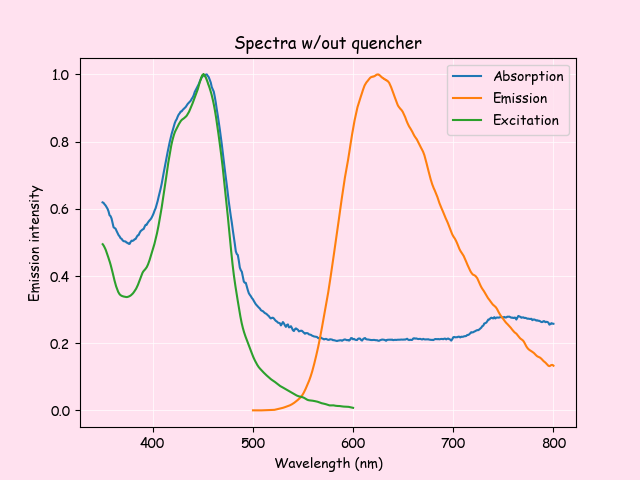
\includegraphics[width = 0.7\linewidth]{part1_noq.png}
    \caption{REDO TITLE}
    \label{fig:enter-label}
\end{figure}
\subsubsection*{In Class Analysis}
\textbf{Question 1} 
\begin{figure}[H]
     \centering
     \begin{subfigure}[b]{0.49\textwidth}
         \centering
         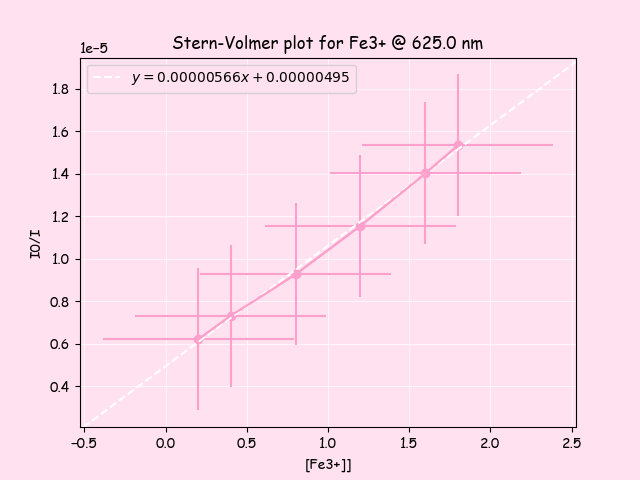
\includegraphics[width=\textwidth]{part1_q1_Fe.png}
         \caption{\ce{Fe^{3+}}}
         \label{fig:part1_q1_fe}
     \end{subfigure}
     \hfill
     \begin{subfigure}[b]{0.49\textwidth}
         \centering
         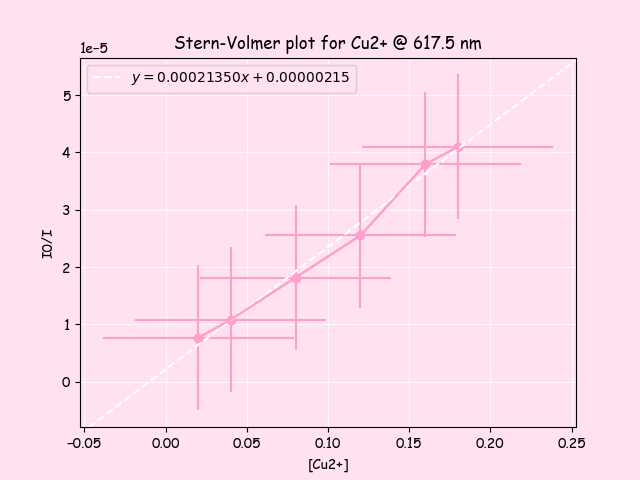
\includegraphics[width=\textwidth]{part1_q1_Cu.png}
         \caption{\ce{Cu^{2+}}}
         \label{fig:part1_q1_Cu}
     \end{subfigure}
     \caption{Stern-Volmer plots for luminescent quenching measurements}
     \label{fig:stern_volmers}
\end{figure}

Figure \ref{fig:stern_volmers} represents the following curve (eqn (6)) from lab manual\autocite{lab_manual}:
\begin{equation*}
    \frac{I_0}{I} = 1 + \frac{k_q}{k_d}[Q]
\end{equation*}

So $\frac{k_q}{k_d}$ is the slope of each curve. So:
\begin{equation*}
    \mathcolorbox{Lavender}{\frac{dy}{dx}_{\text{Fe}^{3+}} = \input{part1_q1_fe_slope.txt} \text{ @ } \input{part1_q1_fe_wl.txt} \text{ nm} }
\end{equation*}
And
\begin{equation*}
    \mathcolorbox{Lavender}{\frac{dy}{dx}_{\text{Cu}^{2+}} = \input{part1_q1_cu_slope.txt} \text{ @ } \input{part1_q1_cu_wl.txt} \text{ nm} }
\end{equation*}
\\
\textbf{Question 2}
\par From the lab manual\autocite{lab_manual}, $k_d = 1.7 \times 10^6\text {s}^{-1}$. Thus,
\begin{equation}
    k_q = \text{slope} \times k_d
    \label{eq:p1q2}
\end{equation}
Substituting slopes to equation (\ref{eq:p1q2}):
\begin{equation*}
    \mathcolorbox{Lavender}{k_{q,\text{Fe}^{3+}} = \input{part1_q2_fe.txt} \text{ s}^{-1}}
\end{equation*}
\begin{equation*}
    \mathcolorbox{Lavender}{k_{q,\text{Cu}^{2+}} = \input{part1_q2_cu.txt} \text{ s}^{-1}}
\end{equation*}
\\
\textbf{Question 3}
\par From tables 2 and 3 in the lab manual\autocite{lab_manual}:
   $ k_{11} = 1 \times 10 ^ 8 \text{ M}^{-1}\text{s}^{-1}$, 
    $k_{22, \text{Fe}^{3+}} = 4 \text{ M}^{-1}\text{s}^{-1}$, 
    $k_{22, \text{Cu}^{2+}} = 1 \times 10 ^ {-5} \text{ M}^{-1}\text{s}^{-1}$. And standard reduction potentials: $E^{\circ}_{\text{R}^{3+}} = -0.8 \text{ V}$, $E^{\circ}_{\text{Fe}^{3+}} = 0.77 \text{ V}$, $E^{\circ}_{\text{Cu}^{2+}} = 0.16 \text{ V}$.
\\ Since $E^{\circ}_{\text{Cell}} = E^{\circ}_{\text{Red}} + E^{\circ}_{\text{Ox}}$, 
\begin{equation}
    E^{\circ}_{\text{Cell}} = E^{\circ}_{\text{Red}} + 0.8 \text{ V}
    \label{eq:ecell}
\end{equation}
Rearranging equations (13) and (12) respectively from the lab manual\autocite{lab_manual},
\begin{equation}
    K_{12} = e^{\frac{zF}{RT}E^{\circ}_{\text{Cell}}}
    \label{eq:K12}
\end{equation}
\begin{equation}
    f_{12} = e^{\frac{(\ln{K_{12}})^2}{4\ln{(k_{11}k_{22} / Z_{12}^2)}}}
    \label{eq:f12}
\end{equation}
Equation (11) from the lab manual\autocite{lab_manual} gives:
\begin{equation}
    k_{\text{ET}} = k_{12} \approx \sqrt{k_{11}k_{22}K_{12}f_{12}}
    \label{eq:ket}
\end{equation}
Where $Z_{12} \approx 10^{11} \text{ M}^{-1} \text{s}^{-1}$, $T = 298.15\text{ K}$, $R = 8.3145\text{ Jmol}^{-1}\text{K}^{-1}$and $F = 96485.3399 \text{ Cmol}^{-1}$.
\\
\par The below Python function (see Appendix \ref{appx:part1_code} for full script) takes inputs for ($k_{22}$, $E^{\circ}_{\text{Red}}$, $z$), and substitutes above given values, equations (\ref{eq:ecell}), (\ref{eq:K12}), and (\ref{eq:f12}) to equation (\ref{eq:ket}), to return the $k_{\text{ET}}$ value.
\input{marcus_theory_fn.txt}
This function was called for ($k_{22 \text{Fe}^{3+}}$, $E^{\circ}_{\text{Fe}^{3+}}$, $z = 3$), and ($k_{22, \text{Cu}^{2+}}$, $E^{\circ}_{\text{Cu}^{2+}}$, $z = 2$) to respectively return
\begin{equation*}
    \mathcolorbox{Lavender}{k_{\text{ET},\text{Fe}^{3+}} = \input{part1_q3_fe.txt} \text{ M}^{-1} \text{s}^{-1}}
\end{equation*}
\begin{equation*}
    \mathcolorbox{Lavender}{k_{\text{ET},\text{Cu}^{2+}} = \input{part1_q3_cu.txt} \text{ M}^{-1} \text{s}^{-1}}
\end{equation*}

\subsubsection*{Discussion Questions}

\subsection{Part 2}





